\subsection{Appendices}

Appendix A. Character Sheet

106

\begin{table}
\begin{tabular}{|l|l|} \hline 
\multicolumn{2}{|l|}{\textbf{Player details}} \\
 \hline Name: & Phone number: \\
 \hline \multicolumn{2}{|l|}{Address:} \\
 \hline \multicolumn{2}{|l|}{Postcode:} \\
 \hline  Date of birth:/	/ & Email: \\
 \hline \multicolumn{2}{|l|}{Medical conditions / allergies:} \\
 \hline Emergency contact name: & Emergency contact phone number: \\
 \hline \end{tabular}

\end{table}

\begin{table}
\begin{tabular}{|l|l|l|l|l|} \hline 
\multicolumn{5}{|l|}{\textbf{Character details}} \\
 \hline \multirow{1}{*}{Name:}& Awareness & 1 / 2 / 3 & Melee Weapons & 1 / 2 / 3 \\
\cline{2-2}\cline{3-3}\cline{4-4}\cline{5-5} & Backstab & 1 / 2 / 3 & Omega Body & 1 / 2 / 3 \\
 \hline \multirow{1}{*}{Race:}& Bulging Biceps & 1 / 2 / 3 & Omega Energy & 1 / 2 / 3 \\
\cline{2-2}\cline{3-3}\cline{4-4}\cline{5-5} & Courage & 1 / 2 / 3 & Omega Mind & 1 / 2 / 3 \\
 \hline \multirow{1}{*}{Regiment:}& Dodge & 1 / 2 / 3 & Omega Protection & 1 / 2 / 3 \\
\cline{2-2}\cline{3-3}\cline{4-4}\cline{5-5} & Engineering & 1 / 2 / 3 & Omega Spirit & 1 / 2 / 3 \\
 \hline \multirow{1}{*}{Rank:}& Explosives & 1 / 2 / 3 & Pharmacology & 1 / 2 / 3 \\
\cline{2-2}\cline{3-3}\cline{4-4}\cline{5-5} & Extra Hits & 1 / 2 / 3 & Pistol & 1 / 2 / 3 \\
 \hline \multirow{1}{*}{Class:}& Focus & 1 / 2 / 3 & Rifle & 1 / 2 / 3 \\
\cline{2-2}\cline{3-3}\cline{4-4}\cline{5-5} & Heavy Weapons & 1 / 2 / 3 & Self-Sufficient & 1 / 2 / 3 \\
 \hline \multirow{1}{*}{Home planet:}& Marksman & 1 / 2 / 3 & Stealth & 1 / 2 / 3 \\
\cline{2-2}\cline{3-3}\cline{4-4}\cline{5-5} & Medicae & 1 / 2 / 3 & Veteran picks &  \\
 \hline \end{tabular}

\end{table}

	Trinity Games understands the requirements of the Data Protection Act (1998) and will not pass any personal information to third parties. Personal information given will be treated in the strictest confidence, and only those who need to know (such as event management and medical staff) will have access to it. If you do not wish your personal data (except contact data) to be held while you are an active customer, please place an X within the brackets.{[} {]}

\begin{table}
\begin{tabular}{|l|l|l|l|} \hline 
\multicolumn{4}{|l|}{\textbf{For Game Organisation Desk (GOD) use only}} \\
 \hline Player ID: & Med code: & Database: & Event: \\
 \hline \end{tabular}

\end{table}

\begin{table}
\begin{tabular}{|l|l|l|l|l|l|l|} \hline 
\textbf{Character card} & \multicolumn{6}{|l|}{\textbf{Player name:}} \\
 \hline Name: & Awareness &  & Focus &  & Omega Protect &  \\
 \hline Race: & Backstab &  & Heavy Weapons &  & Omega Spirit &  \\
 \hline Regiment: & Bulging Biceps &  & Marksman &  & Pharmacology &  \\
 \hline Rank: & Courage &  & Medicae &  & Pistol &  \\
 \hline Class: & Dodge &  & Melee Weapons &  & Rifle &  \\
 \hline Home planet: & Engineering &  & Omega Body &  & Self-Sufficient &  \\
 \hline Player ID: & Explosives &  & Omega Energy &  & Stealth &  \\
 \hline Medical code: & Extra Hits &  & Omega Mind &  & Veteran picks &  \\
 \hline \end{tabular}

\end{table}
Appendix B. Skill Times - Stabilise, Heal, Repair, Marksman

\subsection{Stabilise}

\begin{table}
\begin{tabular}{|l|l|l|l|} \hline 
\multirow{1}{*}{}& \multicolumn{3}{|l|}{Stabilisation times using Medicae skill (in seconds)} \\
\cline{2-2}\cline{3-3}\cline{4-4} & Tier 1 & Tier 2 & Tier 3 \\
 \hline Alone & 30 & 25 & 20 \\
 \hline 1 assistant & 25 & 20 & 15 \\
 \hline 2 assistants & 20 & 15 & 10 \\
 \hline \end{tabular}

\end{table}

\textbf{Heal}

\begin{table}
\begin{tabular}{|l|l|l|l|} \hline 
\multirow{1}{*}{}& \multicolumn{3}{|l|}{Heal times using Medicae skill (in seconds)} \\
\cline{2-2}\cline{3-3}\cline{4-4} & Tier 1 & Tier 2 & Tier 3 \\
 \hline Alone & 100 & 80 & 60 \\
 \hline 1 assistant & 80 & 60 & 40 \\
 \hline 2 assistants & 60 & 40 & 30 \\
 \hline \end{tabular}

\end{table}

\textbf{Repair}

\begin{table}
\begin{tabular}{|l|l|l|l|} \hline 
\multirow{1}{*}{}& \multicolumn{3}{|l|}{Armour repair times using the Engineering skill (in seconds)} \\
\cline{2-2}\cline{3-3}\cline{4-4} & Tier 1 & Tier 2 & Tier 3 \\
 \hline \multicolumn{4}{|l|}{No engineering skill:180} \\
 \hline Alone & 100 & 80 & 60 \\
 \hline 1 assistant & 80 & 60 & 40 \\
 \hline 2 assistants & 60 & 40 & 30 \\
 \hline \end{tabular}

\end{table}

\textbf{Marksman}

\begin{table}
\begin{tabular}{|l|l|l|l|} \hline 
\multirow{1}{*}{}& \multicolumn{3}{|l|}{Aiming times for Cripple and Marksman call using the Marksman skill (in seconds)} \\
\cline{2-2}\cline{3-3}\cline{4-4} & Tier 1 & Tier 2 & Tier 3 \\
 \hline Cripple call & 40 & 35 & 30 \\
 \hline Cripple call + Sniper class & 35 & 30 & 25 \\
 \hline Marksman call & 45 & 40 & 35 \\
 \hline Marksman call + Sniper class & 40 & 35 & 30 \\
 \hline \end{tabular}

\end{table}

\textbf{Appendix C. Class Primary Skills, Secondary Skills, Armour and Starting Skill Points}

*Mandatory free starting skills.

**Starting skill options, choose one marked with ** at Tier 1 at character creation.

***Starting skill points.

\begin{table}
\begin{tabular}{|l|l|l|l|l|} \hline 
Class & Primary skills & Secondary skills & Max armour & SSP*** \\
 \hline Adept & Melee & Awareness & Light & 3 \\
 \hline \textit{pp. 55} & Omega Attunement 1* & Courage &  &  \\
 \hline  & Omega Attunement 2 & Omega Attunement 3 &  &  \\
 \hline  & Pistol &  &  &  \\
 \hline Engineer & Engineering* & Awareness & Medium & 2 \\
 \hline \textit{pp. 56} & Explosives & Extra Hits &  &  \\
 \hline  & Pistol & Rifle &  &  \\
 \hline  & Self-sufficient &  &  &  \\
 \hline  & Regimental specialisation* &  &  &  \\
 \hline Heavy Weapons & Bulging Biceps & Courage & Heavy & 2 \\
 \hline Specialist & Extra Hits** & Explosives &  &  \\
 \hline \textit{pp. 56} & Heavy Weapons** & Pistol &  &  \\
 \hline  & Melee** &  &  &  \\
 \hline  & Regimental specialisation* &  &  &  \\
 \hline Medic & Courage & Bulging Biceps & Medium & 2 \\
 \hline \textit{pp. 57} & Medicae* & Extra Hits &  &  \\
 \hline  & Pharmacology & Rifle &  &  \\
 \hline  & Pistol &  &  &  \\
 \hline  & Regimental specialisation* &  &  &  \\
 \hline Scout & Awareness & Dodge & Medium & 2 \\
 \hline \textit{pp. 58} & Backstab** & Pistol &  &  \\
 \hline  & Self-sufficient & Rifle &  &  \\
 \hline  & Stealth** &  &  &  \\
 \hline  & Regimental specialisation* &  &  &  \\
 \hline Sniper & Awareness & Courage & Medium & 1 \\
 \hline \textit{pp. 59} & Marksman* & Dodge &  &  \\
 \hline  & Rifle* & Pistols &  &  \\
 \hline  & Stealth &  &  &  \\
 \hline  & Regimental specialisation* &  &  &  \\
 \hline Trooper & Courage & Bulging Biceps & Heavy & 2 \\
 \hline \textit{pp. 59} & Dodge** & Pistol &  &  \\
 \hline  & Melee** & Self-sufficient &  &  \\
 \hline  & Rifle** &  &  &  \\
 \hline  & Regimental specialisation* &  &  &  \\
 \hline Mascen Big'un & Bulging Biceps** & Explosives & Heavy & 3 \\
 \hline \textit{pp. 60} & Courage & Self-sufficient &  &  \\
 \hline  & Extra Hits & Rifle &  &  \\
 \hline  & Melee** &  &  &  \\
 \hline Mascen Little'un & Dodge & Awareness & Medium & 3 \\
 \hline Shaman & Omega Spirit Attunement* & Omega Attunement 3 &  &  \\
 \hline \textit{pp. 60} & Omega Attunement 2 & Pistol &  &  \\
 \hline  & Self-sufficient &  &  &  \\
 \hline Mascen Little'un & Dodge & Awareness & Medium & 3 \\
 \hline Tinkerer & Engineering** & Explosives &  &  \\
 \hline \textit{pp. 61} & Pistol & Rifle &  &  \\
 \hline  & Self-sufficient** &  &  &  \\
 \hline \end{tabular}

\end{table}

\begin{table}
\begin{tabular}{|l|l|l|l|l|} \hline 
Myr'na Healer & Extra Hits & Awareness & Light & 3 \\
 \hline \textit{pp. 62} & Medicae & Courage &  &  \\
 \hline  & Omega Body Attunement* & Omega Attunement 3* &  &  \\
 \hline  & Omega Attunement 2 &  &  &  \\
 \hline Myr'na Warrior & Courage & Bulging Biceps & Medium & 3 \\
 \hline \textit{pp. 63} & Extra Hits & Heavy Weapons &  &  \\
 \hline  & Medicae & Rifle &  &  \\
 \hline  & Melee* &  &  &  \\
 \hline Tae'go & Backstab & Dodge & Medium & 3 \\
 \hline \textit{pp. 64} & Pharmacology** & Medicae &  &  \\
 \hline  & Self-sufficient & Rifle &  &  \\
 \hline  & Stealth** &  &  &  \\
 \hline Vrede & Courage & Melee & None & 3 \\
 \hline \textit{pp. 65} & Dodge & Pistol &  &  \\
 \hline  & Engineering** & Self-sufficient &  &  \\
 \hline  & Rifle** &  &  &  \\
 \hline \end{tabular}

\end{table}

Appendix D. Skill Points Costs

The skill point costs for primary skills are as follows:

\begin{table}
\begin{tabular}{|l|l|l|} \hline 
\multicolumn{3}{|l|}{Primary skill costs} \\
 \hline Tier 1 & Tier 2 & Tier 3 \\
 \hline 1 & 2 & 3 \\
 \hline \end{tabular}

\end{table}

The skill point costs for secondary skills are as follows:

\begin{table}
\begin{tabular}{|l|l|l|} \hline 
\multicolumn{3}{|l|}{Secondary skill costs} \\
 \hline Tier 1 & Tier 2 & Tier 3 \\
 \hline 2 & 3 & 4 \\
 \hline \end{tabular}

\end{table}

The skill point costs for veteran picks are as follows:

\begin{table}
\begin{tabular}{|l|l|l|l|} \hline 
Skill type & Tier 1 & Tier 2 & Tier 3 \\
 \hline 1st veteran pick & 2 & - & - \\
 \hline 2nd veteran pick & 3 & 3 & - \\
 \hline 3rd veteran pick & 4 & 4 & 4 \\
 \hline 4th veteran pick & 5 & 5 & 5 \\
 \hline 5th veteran pick & 6 & 6 & 6 \\
 \hline 6th veteran pick & 7 & 7 & 7 \\
 \hline 7th veteran pick & 8 & 8 & 8 \\
 \hline 8th veteran pick & 9 & 9 & 9 \\
 \hline 9th veteran pick & 10 & 10 & 10 \\
 \hline 10th veteran pick & 11 & 11 & 11 \\
 \hline \end{tabular}

\end{table}

Appendix E. Crafting and Components Lists: Engineering

Known components and their rarity

\begin{table}
\begin{tabular}{|l|l|l|} \hline 
Common & Uncommon & Rare \\
 \hline Circuit board Fabric Gears\par Glass Gunpowder Metal\par Oil Tubing Wiring Wood & Battery Gunparts Liquid gas Motor\par Organic circuits Radio transmitter Refined oil & Emitter unit Powerpack Scanner Sensor Thermoplasma \\
 \hline \end{tabular}

\end{table}

\textbf{Standard Engineering crafting list}

*Vrede only without research

\begin{table}
\begin{tabular}{|l|l|l|l|l|} \hline 
Tech name & Components & EWP & Maintenance & Effect \\
 \hline Bionic limb & 1 x Organic circuits 1 x Gears\par 1 x Wiring\par 1 x Metal & 2 & N/a &  \\
 \hline Blind grenade & 1 x Gunpowder\par 1 x Tubing\par 1 x Oil\par 1 x Glass & 2 & 1 year & Causes the Blind call on nearest 2 people within 10 feet, after being thrown. \\
 \hline Frag grenade & 1 x Gunpowder\par 1 x Tubing\par 1 x Metal\par 1 x Oil & 2 & 1 year & Causes the Blast call on nearest 2 people within 10 feet, after being thrown. \\
 \hline Light energy shield* & 

x Emitter unit 2 x Battery

x Radio transmitter 4 x Circuit board

4 x Wiring


 & 8 & 1 year & 2 global hits, regenerates 50\% of total hits per encounter. May wait for two encounters to fully regenerate all hits. \\
 \hline Light patterned armour - Arms & 3 x Fabric\par 2 x Metal\par 1 x Wood & 2 & 2 years & Light armour with 2 armour hits on each arm. \\
 \hline Light patterned armour - Full set & 1 x Refined oil\par 10 x Fabric\par 6 x Metal\par 5 x Wood & 7 & 2 years & Light armour with 2 armour hits on every location. \\
 \hline Light patterned armour - Head & 2 x Fabric\par 2 x Metal\par 1 x Wood & 2 & 2 years & Light armour with 2 armour hits on the head. \\
 \hline Light patterned armour - Legs & 3 x Fabric\par 2 x Metal\par 1 x Wood & 2 & 2 years & Light armour with 2 armour hits on each leg. \\
 \hline Light patterned armour - Torso &
x Refined oil

x Fabric

1 x Metal\par 1 x Wood & 2 & 2 years & Light armour with 2 armour hits on the torso. \\
 \hline \end{tabular}

\end{table}

\begin{table}
\begin{tabular}{|l|l|l|l|l|} \hline 
Liquid gas & 1 x Wood\par 1 x Gunpowder\par 1 x Fabric\par 1 x Glass & 1 & N/a &  \\
 \hline Marksman round & 1 x Gunpowder\par 1 x Metal & 1 & N/a & Allows use of the marksman skill. \\
 \hline Multispectrum systems analyser &

x Wiring

x Circuit board 1 x Metal

 & 4 & N/a & Allows various additional engineering abilities. Genetically keyed to creator, will not function after their death. Please see ppxx for more details. \\
 \hline Organic circuits & 1 x Wiring\par 1 x Circuit board 1 x Fabric\par 1 x Glass & 1 & N/a &  \\
 \hline Refined oil & 1 x Wood\par 1 x Oil\par 1 x Fabric\par 1 x Tubing & 1 & N/a &  \\
 \hline Rifle bipod & 1 x Gun parts 1 x Gears\par 1 x Metal 1x Tubing & 3 & 1 year & Reduce times required for calls made using the Marksman skill by 5 seconds. Bipod must be deployed on a solid surface for use. \\
 \hline Standard laboratory & 1 x Powerpack\par 1 x Battery\par 1 x Liquid gas\par 1 x Organic circuits\par 1 x Refined oil\par 3 x Glass\par 2 x Wood\par 2 x Oil\par 2 x Fabric\par 2 x Tubing\par 1 x Metal\par 1 x Wiring\par 1 x Circuit board & 18 & 2 years & Required for Pharmacology research, grants no PWP bonus.\par This laboratory can be used for two research projects a day.\par \textbf{PWP} may be spent to craft this item if it is crafted by a character with the Pharmacology skill. \\
 \hline Standard workbench & 1 x Powerpack\par 1 x Battery\par 1 x Motor\par 1 x Radio transmitter 1 x Gun parts\par 3 x Gears\par 2 x Wood\par 2 x Oil\par 2 x Metal\par 2 x Tubing\par 1 x Fabric\par 1 x Wiring\par 1 x Circuit board & 18 & 2 years & Required for Engineering research, grants no EWP bonus.\par This workbench can be used for 2 research projects a day. \\
 \hline Static turret mount & 1 x Gunparts\par 1 x Motor\par 3 x Gears\par 2 x Wood\par 2 x Oil\par 2 x Metal & 6 & 1 year & When placed on a statuic base, allows use of a heavy weapon without the skill. Mount can be moved, requires extreme effort and manpower to do so. \\
 \hline \end{tabular}

\end{table}

Advanced Engineering crafting list

*Vrede only without research

\begin{table}
\begin{tabular}{|l|l|l|l|l|} \hline 
Tech name & Components & EWP & Maintenance & Effect \\
 \hline Advanced laboratory & Standard laboratory 1 x Scanner\par

x Sensor 2x Battery

x Liquid gas

2 x Organic circuits\par 2 x Refined oil\par 1 x Motor\par 3 x Glass\par 2 x Wood\par 2 x Oil\par 2 x Fabric\par 2 x Tubing\par 1 x Metal\par 1 x Wiring\par 1 x Circuit board & 20 & 2 years & Required for Pharmacology research, grants 2 PWP bonus.\par This laboratory can be used for two research projects a day, but only one can receive the PWP bonus.\par \textbf{PWP} may be spent to craft this item if it is crafted by a character with the Pharmacology skill. \\
 \hline Advanced workbench & Standard workbench 1 x Scanner\par

x Sensor

x Battery

2 x Motor\par 2 x Radio transmitter 2 x Gun parts\par

x Liquid gas 3 x Gears

x Wood

2 x Oil\par 2 x Metal\par 2 x Tubing\par 1 x Fabric\par 1 x Wiring\par 1 x Circuit board & 20 & 2 years & Required for Engineering research, grants 2 EWP bonus.\par This workbench can be used for two research projects a day, but only one can receive the EWP bonus. \\
 \hline Battery & 1 x Circuit board 1 x Oil\par 1 x Gears\par 1 x Wiring & 1 & N/a &  \\
 \hline Gunparts & 1 x Gunpowder\par 1 x Wiring\par 1 x Metal\par 1 x Gears & 1 & N/a &  \\
 \hline Medium energy shield* & Light energy shield 1 x Powerpack\par

x Thermoplasma

x Battery

2 x Radio transmitter 1 x Liquid gas\par 1 x Motor\par 4 x Circuit board 4 x Wiring & 10 & 1 year & 4 global hits, regenerates 50\% of total hits per encounter. May wait for two encounters to fully regenerate all hits. \\
 \hline \end{tabular}

\end{table}

\begin{table}
\begin{tabular}{|l|l|l|l|l|} \hline 
Medium patterned armour - Arms &

x Refined oil

x Metal

2 x Oil\par 1 x Wood\par 1 x Fabric & 4 & 2 years & Medium armour with 3 armour hits on each arm. \\
 \hline Medium patterned armour - Full set & 4 x Refined oil\par 8 x Metal\par 7 x Oil\par 4 x Fabric\par 3 x Wood & 14 & 2 years & Medium armour with 3 armour hits on every location. \\
 \hline Medium patterned armour - Head &

x Refined oil

x Metal

1 x Oil\par 1 x Fabric & 4 & 2 years & Medium armour with 3 armour hits on the head. \\
 \hline Medium patterned armour - Legs &

x Refined oil

x Metal

2 x Oil\par 1 x Wood\par 1 x Fabric & 4 & 2 years & Medium armour with 3 armour hits on each leg. \\
 \hline Medium patterned armour - Torso &

x Refined oil

x Metal

x Fabric

x Oil

1 x Wood & 4 & 2 years & Medium armour with 3 armour hits on the torso. \\
 \hline Motor & 1 x Gears\par 1 x Oil\par 1 x Metal\par 1 x Tubing & 1 & N/a &  \\
 \hline Radio transmitter & 1 x Glass\par 1 x Tubing\par 1 x Metal\par 1 x Circuit board & 1 & N/a &  \\
 \hline Scope &

x Gun parts 2 x Tubing

x Glass

2 x Metal & 4 & 1 year & Minus 5 seconds required for calls made with the Marksman skill.\par Allows use of Marksman skill with heavy weapons. \\
 \hline Shatter grenade & 3 x Gunpowder\par 2 x Gears\par 1 x Oil\par 1 x Glass & 3 & 1 year & Causes Shatter call on 2 chosen close objects within 10 feet, after being thrown. \\
 \hline Shotgun attachment &

x Gun parts 1 x Tubing

x Metal

 & 2 & 1 year & Allows shotgun-style attachments that can be added to rifles or heavy weapons. \\
 \hline Stun grenade & 3 x Gunpowder\par 2 x Wiring\par 2 x Circuit board & 3 & 1 year & Causes Stun and Knockdown call on 2 nearest people within 10 feet, after being thrown. \\
 \hline \end{tabular}

\end{table}

Expert Engineering crafting list

*Vrede only without research

\begin{table}
\begin{tabular}{|l|l|l|l|l|} \hline 
Tech name & Components & EWP & Maintenance & Effect \\
 \hline Expert laboratory & Advanced laboratory 2 x Thermoplasma\par

x Powerpack 1 x Emitter unit 2 x Liquid gas

x Organic circuits

2 x Refined oil\par 1 x Motor\par 3 x Glass\par 2 x Wood\par 2 x Oil\par 2 x Fabric\par 2 x Tubing\par 1 x Metal\par 1 x Wiring\par 1 x Circuit board & 22 & 2 years & Required for Pharmacology research, grants 4 PWP bonus.\par This laboratory can be used for two research projects a day, but only one can receive the PWP bonus.\par \textbf{PWP} may be spent to craft this item if it is crafted by a character with the Pharmacology skill. \\
 \hline Expert workbench & Advanced workbench 2 x Thermoplasma\par

x Powerpack 1 x Emitter unit 2 x Motor

x Radio transmitter 2 x Gun parts

x Liquid gas 3 x Gears

x Wood

2 x Oil\par 2 x Metal\par 2 x Tubing\par 1 x Fabric\par 1 x Wiring\par 1 x Circuit board & 22 & 2 years & Required for Engineering research, grants 4 EWP bonus.\par This workbench can be used for two research projects a day, but only one can receive the EWP bonus. \\
 \hline Grenade launcher attachment & 2 x Gun parts 2 x Tubing\par 4 x Metal & 6 & 1 year & Attachment for heavy weapons or rifles. Allows use of rifle grenades in launcher. \\
 \hline Heavy energy shield* & Medium energy shield 1 x Emitter\par 2 x Thermoplasma\par 2 x Battery\par 2 x Radio transmitter 1 x Liquid gas\par 1 x Motor\par 4 x Circuit board 4 x Wiring & 12 & 1 year & 6 global hits, regenerates 50\% of total hits per encounter. May wait for two encounters to fully regenerate all hits. \\
 \hline Heavy patterned armour - Arms & 1 x Refined oil\par

x Motor

x Metal

2 x Oil\par 2 x Wood & 6 & 2 years & Heavy armour with 4 armour hits on each arm. \\
 \hline \end{tabular}

\end{table}

\begin{table}
\begin{tabular}{|l|l|l|l|l|} \hline 
Heavy patterned armour - Full set & 4 x Refined oil\par 4 x Motor\par 9 x Meta
\setcounter{enumi}{6}

x Oil

x Wood

 & 22 & 2 years & Heavy armour with 4 armour hits on every location. \\
 \hline Heavy patterned armour - Head & 1 x Refined oi

x Motor

x Metal

x Oil

x Wood

 & 6 & 2 years & Medium armour with 4 armour hits on the head. \\
 \hline Heavy patterned armour - Legs & 1 x Refined oil\par

x Motor

x Metal

2 x Oil\par 2 x Wood & 6 & 2 years & Heavy armour with 4 armour hits on each leg. \\
 \hline Heavy patterned armour - Torso & 1 x Refined oil\par 1 x Motor\par 3 x Metal\par 2 x Oil\par 2 x Wood & 6 & 2 years & Heavy armour with 4 armour hits on the torso. \\
 \hline Laser sight & 2 x Gun parts 2 x Tubing\par 2 x Glass\par 2 x Metal & 6 & 1 year & Minus 10 seconds required for calls made with the Marksman skill. Allows use of Marksman skill with heavy weapons. \\
 \hline Poison grenade & Pharmaceutical\par 1 x Organic circuits 2 x Glass\par 1 x Metal\par 1 x Circuit board & 4 & 1 year & Causes the effect of the pharmaceutical added to the closest two people within 10 feet, after being thrown. Note, not all pharmaceuticals are compatible with this tech. \\
 \hline Remote detonator & 1 x Radio transmitter 1 x Circuit board\par 1 x Wiring & 3 & 1 year & Can be attached to explosives to allow remote detonation using a linked multispec. Cannot be removed once attached. \\
 \hline Rifle grenade & 2 x Gunpowder\par 1 x Metal\par 1 x Circuit board & 1 & 6 months & Can only be used in grenade launcher attachments\par Causes Blast call on two closest people within 10 feet, after being launched. \\
 \hline \end{tabular}

\end{table}

Appendix F. Crafting and Ingredients Lists: Pharmacology

Rarity and primary properties of ingredients

\begin{table}
\begin{tabular}{|l|l|l|} \hline 
Ingredient & Rarity & Primary property \\
 \hline Clawhorn & Rare & Necrosis \\
 \hline Curdleclove & Common & Weakness \\
 \hline Dawn Seed & Common & Slowed reactions \\
 \hline Dragon Hazel & Uncommon & Increased heart rate \\
 \hline Forager's Folly & Uncommon & Chameleonic \\
 \hline Greenweald & Common & Regeneration \\
 \hline Moonbark & Uncommon & Luminescent \\
 \hline Morning Leaf & Rare & Headache \\
 \hline Nightweed & Uncommon & Clear mind \\
 \hline Pink Damsel & Common & Dulled senses \\
 \hline Root of Viskeri & Rare & Increased reactions \\
 \hline Sprig-fist & Uncommon & Enhanced senses \\
 \hline Sunbright & Common & Slowed heart rate \\
 \hline Ubria Grass & Common & Toughness \\
 \hline \end{tabular}

\end{table}

\textbf{Standard Pharmacology crafting list}

\begin{table}
\begin{tabular}{|l|l|l|l|l|} \hline 
Pharmaceutical & Components & PWP & Expiry & Effect \\
 \hline Dermagraft patch & 2 x Ubria Grass 2 x Greenweald & 2 & N/a & Applied to the skin, instantly applies the stabilise call to a dying character. \\
 \hline Stunning blade venom & 3 x Curdleclove 2 x Pink Damsel & 3 & 1 year & Applied to melee weapons. Lasts 2 hours once applied. First 2 strikes with the weapon cause the Stun call. \\
 \hline Standard blue chem & 1 x Nightweed & 2 & 1 year & Grants 2 FP to the user. Only 1 blue chem pharmaceutical can be used per day. \\
 \hline Standard courage potion & 2 x Pink Damsel 1 x Ubria Grass 1 x Dawn Seed & 2 & 1 year & Grants the ability to resist a total of 1 Fear call used against the user that day. \\
 \hline Standard healing potion & 2 x Greenweald 2 x Ubria Grass 1 x Sunbright & 3 & 1 year & Restores 1 body hit to all locations 30 seconds after being consumed. \\
 \hline Standard healing syringe & 2 x Greenweald 1 x Ubria Grass & 1 & 1 year & Restores 1 body hit to 1 location instantly. \\
 \hline \end{tabular}

\end{table}

\begin{table}
\begin{tabular}{|l|l|l|l|l|} \hline 
Standard laboratory & 1 x Powerpack\par 1 x Battery\par 1 x Liquid gas\par 1 x Organic circuits\par 1 x Refined oil\par 3 x Glass\par 2 x Wood\par 2 x Oil\par 2 x Fabric\par 2 x Tubing\par 1 x Metal\par 1 x Wiring\par 1 x Circuit board & 18 & 2 years (requires maintenance as per the Engineering skill, may be performed with PWP. See \textit{pp. 92}) & Required for Pharmacology research, grants no PWP bonus.\par This laboratory can be used for two research projects a day.\par \textbf{EWP} may be spent to craft this item if it is crafted by a character with the Engineering skill. \\
 \hline Standard Omega resistance potion & 1 x Nightweed 1 x Ubria Grass & 3 & 1 year & Grants the ability to negate a total of 3 FP of Omega Attunement powers used against user that day. \\
 \hline \end{tabular}

\end{table}

\textbf{Advanced Pharmacology crafting list}

\begin{table}
\begin{tabular}{|l|l|l|l|l|} \hline 
Pharmaceutical & Components & PWP & Expiry & Effect \\
 \hline Advanced blue chem & 2 x Nightweed & 3 & 1 year & Grants 4 FP to user. Only 1 blue chem pharmaceutical can be used per day. \\
 \hline Advanced courage potion & 2 x Pink Damsel 2 x Ubria Grass 2 x Dawn Seed & 3 & 1 year & Grants the ability to resist a total of 2 Fear calls used against the user that day. \\
 \hline Advanced healing potion & 3 x Greenweald 3 x Ubria Grass 2 x Sunbright & 4 & 1 year & Restores 2 body hits to all locations 30 seconds after being consumed. \\
 \hline Advanced healing syringe & 4 x Greenweald 1 x Ubria Grass & 2 & 1 year & Restores 2 body hits to 1 location instantly. \\
 \hline Advanced laboratory & Standard laboratory 1 x Scanner\par

x Sensor 2x Battery

x Liquid gas

2 x Organic circuits\par 2 x Refined oil\par 1 x Motor\par 3 x Glass\par 2 x Wood\par 2 x Oil\par 2 x Fabric\par 2 x Tubing\par 1 x Metal\par 1 x Wiring\par 1 x Circuit board & 20 & 2 years (requires maintenance as per the Engineering skill, may be performed with PWP. See \textit{pp. 92}.) & Required for Pharmacology research, grants 2 PWP bonus.\par This laboratory can be used for two research projects a day, but only one can receive the PWP bonus.\par \textbf{EWP} may be spent to craft this item if it is crafted by a character with the Engineering skill. \\
 \hline Advanced Omega resistance potion & 1 x Nightweed 3 x Ubria Grass & 4 & 1 year & Grants the ability to negate a total of 5 FP of Omega Attunement powers used against user that day. \\
 \hline Crippling blade venom & 1 x Sprig-fist\par 1 x Dragon Hazel 2 x Curdleclove & 5 & 1 year & Applied to melee weapons. Lasts 2 hours once applied. First 2 strikes with the weapon cause the Cripple call. \\
 \hline \end{tabular}

\end{table}

\textbf{Expert Pharmacology crafting list}

\begin{table}
\begin{tabular}{|l|l|l|l|l|} \hline
Pharmaceutical & Components & PWP & Expiry & Effect \\
 \hline Expert blue chem & 3 x Nightweed & 4 & 1 year & Grants 6 FP to user. Only 1 blue chem pharmaceutical can be used per day. \\
 \hline Expert courage potion &

x Nightweed

x Pink Damsel 2 x Ubria Grass 2 x Dawn Seed

 & 4 & 1 year & Grants the ability to resist a total of 3 Fear calls used against user that day. \\
 \hline Expert healing potion & 1 x Sprig-fist\par 3 x Greenweald 2 x Ubria Grass 2 x Sunbright & 5 & 1 year & Restores 3 body hit to all locations 30 seconds after being consumed. \\
 \hline Expert healing syringe & 1 x Dragon Hazel 2 x Greenweald 2 x Ubria Grass & 3 & 1 year & Restores 3 body hit to 1 location instantly. \\
 \hline Expert laboratory & Advanced laboratory\par 2 x Thermoplasma\par

x Powerpack 1 x Emitter unit 2 x Liquid gas

x Organic circuits

2 x Refined oil\par 1 x Motor\par 3 x Glass\par 2 x Wood\par 2 x Oil\par 2 x Fabric\par 2 x Tubing\par 1 x Metal\par 1 x Wiring\par 1 x Circuit board & 22 & 2 years (requires maintenance as per the Engineering skill, may be performed with PWP. See \textit{pp. 92}.). & Required for Pharmacology research, grants 4 PWP bonus.\par This laboratory can be used for two research projects a day, but only one can receive the PWP bonus.\par \textbf{EWP} may be spent to craft this item if it is crafted by a character with the Engineering skill. \\
 \hline Expert Omega resistance potion & 2 x Nightweed 2 x Ubria Grass & 5 & 1 year & Grants the ability to negate a total of 7 FP of Omega Attunement powers used that day. \\
 \hline Paralysing blade venom & 1 x Clawhorn\par 1 x Dragon Hazel 1 x Sunbright\par 1 x Curdleclove & 6 & 1 year & Applied to melee weapons. Lasts 2 hours once applied. First 2 strikes with the weapon cause the Paralyse call. \\
 \hline \end{tabular}

\end{table}

\textbf{Appendix G. Dart Gun Categories}

\begin{table}
\begin{tabular}{|l|l|l|} \hline 
* & = & Maximum 18-round magazine. \\
 \hline ** & = & Maximum 6-round magazine. \\
 \hline *** & = & Rifle due to size/style. \\
 \hline **** & = & Grenade attachment must be crafted in-game to be used. \\
 \hline \end{tabular}

\end{table}

\begin{table}
\begin{tabular}{|l|l|} \hline 
Blaster & Classification \\
 \hline Air Max 6 & Pistol \\
 \hline Air Tech 1000 & Pistol \\
 \hline Air Tech 2000 & Pistol \\
 \hline Air Tech 3000 & Pistol \\
 \hline Air Tech 4000 & Rifle \\
 \hline Air Tech Jet Squadron & Pistol \\
 \hline Air Tek 8 & Rifle \\
 \hline Alpha Trooper & Rifle* \\
 \hline ArmorShot & One-shot pistol \\
 \hline Auto Tek 20 & Heavy \\
 \hline AutoGrip & One-shot pistol \\
 \hline Backlash & One-shot pistol \\
 \hline Barrel Break & Pistol \\
 \hline Barricade & Heavy \\
 \hline Battle Rig Blaster & One-shot pistol \\
 \hline Belt Blaster & Rifle \\
 \hline Blast Fire & Heavy \\
 \hline Blast Hammer & One-shot pistol \\
 \hline Blow Dart Shooter & One-shot pistol \\
 \hline Boba Fett's Armor & One-shot pistol \\
 \hline Cad Bane Blaster & One-shot pistol \\
 \hline Cam ECS-12 & Heavy \\
 \hline Captain Rex Blaster & One-shot pistol \\
 \hline Centurion & Rifle*** \\
 \hline Chainblazer & Rifle \\
 \hline Chewbacca's Bowcaster & Rifle*** \\
 \hline Clear Shot & One-shot pistol \\
 \hline Clip Blaster 10 & Rifle \\
 \hline Clip Tek & Pistol \\
 \hline Clone Trooper Blaster & One-shot pistol \\
 \hline CommLink II & One-shot pistol \\
 \hline Coral Viper & One-shot pistol \\
 \hline Cougar & Rifle \\
 \hline CrossBolt & Rifle* \\
 \hline Crossbow & Rifle \\
 \hline Crossfire Bow & Rifle*** \\
 \hline CycloneShock & Pistol \\
 \hline Dart Blaster Pen & One-shot pistol \\
 \hline Defender T3 & One-shot pistol \\
 \hline Demolisher 2-In-1 & Heavy**** \\
 \hline Deploy & Rifle* \\
 \hline Derringer & One-shot pistol \\
 \hline Detonator & One-shot pistol \\
 \hline \end{tabular}

\end{table}

\begin{table}
\begin{tabular}{|l|l|} \hline 
Blaster & Classification \\
 \hline Diamondista & One-shot pistol \\
 \hline Doominator & Rifle \\
 \hline Double Barrel & Pistol \\
 \hline Doublestrike & Pistol \\
 \hline Dual & Pistol \\
 \hline Eagle Eye & One-shot pistol \\
 \hline Electric Eel & Pistol \\
 \hline Element & One-shot pistol \\
 \hline Eliminator & One-shot pistol \\
 \hline Energon Blaster & Rifle*** \\
 \hline Expand-a-Blast & Rifle*** \\
 \hline FastBlast & Pistol \\
 \hline Firefly & Rifle*** \\
 \hline Firestrike & One-shot pistol \\
 \hline First Shot & One-shot pistol \\
 \hline Flip \& Fire Gauntlet & Pistol \\
 \hline FlipFury & Rifle \\
 \hline Furyfire & Rifle \\
 \hline Gator & One-shot pistol \\
 \hline General Grievous Blaster & One-shot pistol \\
 \hline Guardian Crossbow & Pistol \\
 \hline GunSmoke & Pistol \\
 \hline Hail-Fire & Heavy \\
 \hline Hammershot & Pistol \\
 \hline Hawk & Rifle \\
 \hline Hawkeye Longshot Bow & One-shot pistol \\
 \hline Heartbreaker Bow & One-shot pistol \\
 \hline Hidden Shot & One-shot pistol \\
 \hline Hornet & Heavy \\
 \hline Hunter & Rifle*** \\
 \hline Hyperfire & Rifle \\
 \hline Iron Flyers & One-shot pistol \\
 \hline Iron Raptor & One-shot pistol \\
 \hline Iron Strike Blaster & Rifle*** \\
 \hline Jaguar & Pistol \\
 \hline Jango Fett Action Set & One-shot pistol \\
 \hline Jolt & One-shot pistol \\
 \hline Laser Fang & One-shot pistol \\
 \hline Lightnin' Blitz & Heavy \\
 \hline Lock `n Load & One-shot pistol \\
 \hline Longshot & Rifle* \\
 \hline Longshot front blaster & One-shot pistol \\
 \hline Longstrike & Rifle* \\
 \hline \end{tabular}

\end{table}

\begin{table}
\begin{tabular}{|l|l|} \hline 
Blaster & Classification \\
 \hline Luke Skywalker's Utility Belt & One-shot pistol \\
 \hline Mad Hornet & One-shot pistol \\
 \hline Magnus & Pistol \\
 \hline Magstrike & Heavy \\
 \hline Maniac & Rifle \\
 \hline Manta Ray & Pistol \\
 \hline Maverick & Pistol \\
 \hline Messenger & Pistol \\
 \hline Micro & One-shot pistol \\
 \hline Mini Mischief & Pistol \\
 \hline Mono Blast & One-shot pistol \\
 \hline Ninja Commando Blaster & Rifle \\
 \hline Nite Finder & One-shot pistol \\
 \hline NitroQuad & One-shot pistol \\
 \hline Optimus Prime Blaster & Rifle*** \\
 \hline Over Under & Rifle \\
 \hline Panther & One-shot pistol \\
 \hline Perceptor & One-shot pistol \\
 \hline Pink Crush & One-shot pistol \\
 \hline Pirate Flintlock & One-shot pistol \\
 \hline Power Web Strike Crossbow & One-shot pistol \\
 \hline Powerbelle & Heavy \\
 \hline PowerClip & Heavy \\
 \hline Predator & Rifle*** \\
 \hline Quick 16 & Rifle \\
 \hline Quickstrike & Pistol \\
 \hline RADS 12 & Rifle \\
 \hline Raider & Rifle* \\
 \hline Rampage & Rifle* \\
 \hline Ramrod & One-shot pistol \\
 \hline Range Master & Rifle*** \\
 \hline Range Shot & One-shot pistol \\
 \hline Rapid Fire & Heavy \\
 \hline Rapid Fire Tek & Rifle*** \\
 \hline Rapid Glow & Rifle* \\
 \hline Rapid Red & Heavy \\
 \hline RapidStrike & Heavy \\
 \hline Ratchet Blast & Pistol \\
 \hline Rattler & Pistol \\
 \hline Rayven & Heavy \\
 \hline Razor Fin & One-shot pistol \\
 \hline Razorbeast & Rifle \\
 \hline Rebel Trooper Blaster & One-shot pistol \\
 \hline Recon with attachments & Rfile* \\
 \hline Recon without attachments & Pistol*** \\
 \hline Reflex & One-shot pistol \\
 \hline Retaliator with attachments & Rifle* \\
 \hline Retaliator without attachments & Pistol** \\
 \hline Rhino-Fire & Heavy \\
 \hline \end{tabular}

\end{table}

\begin{table}
\begin{tabular}{|l|l|} \hline 
Blaster & Classification \\
 \hline RipChord & Heavy \\
 \hline Robo Power & Rifle \\
 \hline Rocketstorm & Pistol \\
 \hline Rogue & Pistol \\
 \hline Rotator X-8 & Rifle \\
 \hline RotoFury & Rifle \\
 \hline RotoTrack & Rifle \\
 \hline Rough Cut & Rifle \\
 \hline Sawtooth & Pistol \\
 \hline Scout & One-shot pistol \\
 \hline Secret Shot & One-shot pistol \\
 \hline Secret Shot II & One-shot pistol \\
 \hline Secret Strike & One-shot pistol \\
 \hline Sharp Shot & One-shot pistol \\
 \hline Sharpshooter & One-shot pistol \\
 \hline Sharpshooter II & One-shot pistol \\
 \hline Shell Shock & Pistol \\
 \hline Side Winder & Rifle \\
 \hline Sidestrike & One-shot pistol \\
 \hline Sledgefire with stock & Rifle*** \\
 \hline Sledgefire without stock & Pistol \\
 \hline Slingback & One-shot pistol \\
 \hline Slingfire & Rifle* \\
 \hline Slingfire DX400 & Pistol \\
 \hline Snapfire 8 & Heavy \\
 \hline Sneak Attacker & One-shot pistol \\
 \hline Sneak Shot & Rifle*** \\
 \hline Spectre with attachments & Rifle*** \\
 \hline Spectre without attachments & Pistol \\
 \hline Speedload 6 & Pistol \\
 \hline Speedswarm & Heavy \\
 \hline Spider-Man vs Venom & Pistol \\
 \hline SplitFire & Pistol \\
 \hline Spylight & Pistol \\
 \hline Stampede & Heavy \\
 \hline Star Shot & One-shot pistol \\
 \hline Star-Lord Quad Blaster & Pistol \\
 \hline Starscream Blaster & Pistol \\
 \hline Stealth & One-shot pistol \\
 \hline Stealthfire Shield & Pistol \\
 \hline Airjet Stinger & One-shot pistol \\
 \hline Stinger & One-shot pistol \\
 \hline Stinging Scarab & One-shot pistol \\
 \hline Stockade & Heavy \\
 \hline Stormfire & One-shot pistol \\
 \hline Strikefire & One-shot pistol \\
 \hline Strongarm (Cyber Stryke Gear) & Pistol \\
 \hline Strongarm & Pistol \\
 \hline Stryfe & Heavy \\
 \hline \end{tabular}

\end{table}

	

\begin{table}
\begin{tabular}{|l|l|} \hline 
Blaster & Classification \\
 \hline SuperMAXX 1500 & Pistol \\
 \hline SuperMAXX 2000 & Pistol \\
 \hline SuperMAXX 25 & Pistol \\
 \hline SuperMAXX 3000 & Rifle*** \\
 \hline SuperMAXX 350 & Pistol \\
 \hline SuperMAXX 5000 & Rifle*** \\
 \hline SuperMAXX 750 & One-shot pistol \\
 \hline Surge 10 & Rifle \\
 \hline Surge 6 & Pistol \\
 \hline Swarmfire & Heavy \\
 \hline Sweet Revenge & Pistol \\
 \hline Switch Shot & One-shot pistol \\
 \hline Switch Shots Max & Pistol \\
 \hline Switch Shots Super & One-shot pistol \\
 \hline Switch Shots Ultra & One-shot pistol \\
 \hline Switchfire & Pistol \\
 \hline T-Rex Tranq Gun & Rifle*** \\
 \hline Tech Target Eliminator & One-shot pistol \\
 \hline Tek 3 & Pistol \\
 \hline Tek 4 & Pistol \\
 \hline Tek 5 & Pistol \\
 \hline Tek 6 & Pistol \\
 \hline Tetra Strike & Pistol \\
 \hline Thunderbow & Pistol \\
 \hline Thundershot & Rifle*** \\
 \hline Torrent & Rifle \\
 \hline Triad & Pistol \\
 \hline Triple Torch & One-shot pistol \\
 \hline Turbo Fire & Rifle \\
 \hline Ultimate Snipe Blast & One-shot pistol \\
 \hline Venom Shot & One-shot pistol \\
 \hline Vigilante & Rifle*** \\
 \hline Vulcan & Heavy \\
 \hline Warthog & One-shot pistol \\
 \hline Whipshot & One-shot pistol \\
 \hline Whiptail Scorpion & Pistol \\
 \hline Wildfire & Heavy \\
 \hline Wrist Blitzer & One-shot pistol \\
 \hline Xcess & Rifle \\
 \hline \end{tabular}

\end{table}

Appendix H. Sample Character Builds

These are designed to give you an insight into the character creation process, and how a character might develop over time. They also highlight some of the features of different classes.

\subsection{Michael Fuller}

\textit{``When you kill, don't think too hard about it. Do your job, do it well, but don't glorify in war. Just survive, and live to enjoy another cup of tea.''}

\begin{table}
\begin{tabular}{|l|l|} \hline 
Name & Michael Fuller \\
 \hline Race & Human (Delmonte) \\
 \hline Regiment & Delmont 205th \\
 \hline Class & Trooper \\
 \hline \end{tabular}

\end{table}

Starting skill points to spend: 2

\textit{Class attributes}

\begin{itemize}
\item \textbf{Tenacious}: Michael receives 2 global hits as per the Dodge skill, without the need for the skill, and it stacks if he purchases the skill.

\item \textbf{Dodged the bullet!}: Once Michael reaches Tier 3 of the Dodge skill he only needs to expend 2 dodge hits to avoid a call instead of all of them.

\item \textbf{Canny}: Once per encounter, Michael may use one additional call

from the Rifle skill, providing he already has the ability to use it. \textit{{[}If Michael purchased the Melee Weapons skill and increased it to Tier 2 he could also apply this attribute to a call from that skill.{]}}

\end{itemize}
\textit{Skills}

\textbf{Self-sufficient} Tier 1 (free regimental specialist skill).

\textbf{Rifle} Tier 2 (free starting class skill, chosen instead of Dodge or Melee Weapons; primary skill, 2 starting skill points spent to increase to Tier 2).

\textit{Hits}

Can wear up to heavy armour. 2 body hits per location.

3 armour hits per armoured location, while wearing heavy armour. 2 global hits, from the Tenacious class attribute.

\textit{Character progression after two events}

Michael receives 2 skill points to spend for every event that he survives.

After his first event, Michael spends 1 point to purchase the \textbf{Courage} skill (primary skill) at Tier 1 and 1 point to purchase the \textbf{Dodge} skill (primary skill) at Tier 1. The Dodge skill grants him an additional 1 global hit, which stacks with his Tenacious class attribute to give him a total of 3 global hits.

After his second event, Michael spends 2 skill points to increase his \textbf{Courage} skill (primary skill) to Tier 2. During his second event Michael is promoted in rank to Sergeant, and given responsibility for a unit of riflemen.

Michael Fuller has joined the Green Cloaks to escape a pretty bad situation back home. Of course, with Delmont as home most things can be pretty bad, but his situation really took the biscuit. If you think that fighting the One Bakkar on the front lines is preferable to home, you know you've got it bad.

Michael is a staunch man, steadfast but weary of the world. He doesn't seem to be bothered by the act of killing another living creature, not even seeming to take any pride in a well-placed shot. It's almost like he's done it too much already, and now it's just old news. Where the younger men in his regiment return from a battle telling tales of their heroics, Michael prefers to make a cup of tea and enjoy it by the fire. But nobody interrupts his tea drinking. Woe to the enemy that attacks during that sacred time!

\subsection{Petrov Ivanovich}

\textit{``I've got all the time in the world, boss.''}

Starting skill points to spend: 1

\textit{Class attributes}

\begin{table}
\begin{tabular}{|l|l|} \hline 
Name & Petrov Ivanovich \\
 \hline Race & Human (Rossii) \\
 \hline Regiment & Kingskeep 98th \\
 \hline Class & Sniper \\
 \hline \end{tabular}

\end{table}

\begin{itemize}
\item \textbf{The Tools for the Job}: Petrov is issued 5 marksman rounds as equipment at the start of every event.

\item \textbf{Keen Eye}: Petrov receives a 5-second reduction on the aiming time when using the Marksman skill.

\item \textbf{Incapacitate the Target}: Once per encounter, Petrov may use the Cripple call as per the Marksman skill, without expending any marksman rounds.

\end{itemize}
\textit{Skills}

\textbf{Stealth} Tier 1 (free regimental specialist skill).

\textbf{Rifle} Tier 1 (free class starting skill).

\textbf{Marksman} Tier 1 (free class starting skill) - it takes him 40 seconds to use the Marksman call, and 35 seconds to use the Cripple call.

\textit{{[}Snipers receive both free class starting skills at character creation, but only receive 1 skill point to spend instead of 2.{]}}

\textbf{Awareness} Tier 1 (primary skill, 1 starting skill point spent).

\textit{Hits}

Can wear up to medium armour. 2 body hits per location.

2 armour hits per armoured location, while wearing medium armour.

\textit{Character progression after two events}

Petrov receives 2 skill points to spend for every event he survives.

After his first event, Petrov spends his 2 skill points to increase his \textbf{Marksman} skill (primary skill) to Tier 2. This means his time required to use the Marksman and Cripple calls has decreased by a further 5 seconds. After his second event, he spends his 2 skill points to increase his \textbf{Rifle} skill (primary skill) to Tier 2, allowing him to use the calls Through or Stun once per encounter.

Growing up on Rossi can be harsh and dangerous. If the bears don't kill you, the vodka, cold, or women might. Every Rossii has his or her own way of surviving, and for Petrov it was to not be seen, stay unnoticed, and just get on with what you're doing. Like many young men he emigrated to Ardheim as soon as he was old enough (whereupon he was disappointed to find that Ardheim also had bears), and not long after enlisted in the Ardheim Defence Force. Showing promise as a rifleman, he was sent for training at the Keep, where due to his patient nature and keen eye he excelled as a sniper. While others in his unit picked up roundshields and melee weapons, heading off into the forests of Ardheim to cut the tree that would become their own shield, Petrov just practiced with his rifle. Eventually he was put forward for the final training and the test of the Keep, which he passed with flying colours{\dots} almost. If it hadn't have been for the bear he'd not have had to take that out first, losing 3 seconds on his time for the actual target. Damn bears. Nevertheless, he was one of the few who passed the training, and was immediately sent to the front lines to serve in Kingskeep 98th.

Dana O'Malley

\textit{``Don't you dare die on me. If you do, I'll kill you!''}

\begin{table}
\begin{tabular}{|l|l|} \hline 
Name & Dana O'Malley \\
 \hline Race & Human (Marazionite) \\
 \hline Regiment & 23rd Heavy Infantry \\
 \hline Class & Medic \\
 \hline \end{tabular}

\end{table}

Starting skill points to spend: 2

\textit{Skills}

\textbf{\textit{Class attributes}}

\begin{itemize}
\item \textbf{Medical Supplies}: Dana is issued with an additional 2 dermograft patches at the start of every event (total 3).

\item \textbf{Medical Researcher}: Dana can undertake Pharmacology research.

\item \textbf{Deathwatch}: Dana can diagnose a dying character, allowing them to tell her what their death count is.

\item \textbf{Triage}: Dana can lead up to 2 other people with the Medicae skill in a triage team to decrease the time it takes to stabilise and heal people.

\end{itemize}
\textbf{Heavy Weapons} Tier 1 (free regimental specialist skill).

\textbf{Medicae} Tier 1 (free starting class skill).

\textbf{Courage} Tier 1 (primary skill, 1 starting skill point spent).

\textbf{Pharmacology} Tier 1 (primary skill, 1 starting skill point spent).

\textit{Hits}

Can wear up to medium armour. 2 body hits per location.

armour hits per armoured location, while wearing medium armour.

\textit{Character progression after two events}

Dana receives 2 skill points to spend for every event that she survives.

She uses the 2 skill points she receives after her first event to increase her \textbf{Medicae} skill to Tier 2, further reducing the time it takes her to stabilise and heal characters. With the 2 skill points she receives after her second event, she purchases \textbf{Bulging Biceps} at Tier 1, a secondary skill for Medics. This allows her to use a shield to protect herself and her patients, but she also intends to increase it to Tier 3 over the next couple of events, to make it easier for her to grapple and move people who are injured away from the front lines.

At her first event Dana is promoted to Sergeant and Chief Medic of the 23rd. At her third event she

becomes Captain of the regiment and passes on the Chief Medic role to a promising recruit.

Dana likes to be good at a great number of things, and indeed she can mow you down in a rain of bullets, craft pharmaceuticals and invent new ones, stitch you up and stop you dying, and what's more is that she is completely unafraid. Little fazes her, and she can routinely be found stomping around the battlefield roughly tending to the wounded, talking frightened soldiers into heading back into the fray, giving orders, and pouring pharmaceuticals down her allies' throats. She accepts no weakness, scolds hesitation, but makes you feel like a big damn hero when you're bleeding out on the ground and she's stitching you up.

\subsection{Krakkt}

\textit{``Here, I bought you the head of the man that looked at you funny yesterday.''}

\begin{table}
\begin{tabular}{|l|l|} \hline 
Name & Krakkt \\
 \hline Race & Mascen \\
 \hline Regiment & Kingskeep 98th \\
 \hline Class & Big'un \\
 \hline \end{tabular}

\end{table}

Starting skill points to spend: 3

\textit{Skills}

\textbf{\textit{Class attributes}}

\begin{itemize}
\item \textbf{Tough Hide}: Krakkt receives 1 extra body hit per location.

\item \textbf{Unwavering}: Krakkt receives 1 extra Fear resist per encounter, as per the Courage skill, without needing the skill.

\item \textbf{Unstoppable}: Twice per day, Krakkt may enter a state of pure rage for 10 seconds, during which all damage taken is delayed until the rage has finished.

\end{itemize}
\textbf{Melee} Tier 1 (free class starting skill).

\textbf{Courage} Tier 2 (primary skill, 1 starting skill point spent to purchase Tier 1, 2 starting skill points spent to increase to Tier 2).

\textit{Hits}

May wear up to heavy armour.

body hits per location (2 standard, 1 extra from Tough Hide class attribute). 3 armour hits per armoured location, while wearing heavy armour.

\textit{Character progression after two events}

Krakkt receives 2 skill points to spend for each event she survives.

She chooses to spend her first 2 skill points to increase her \textbf{Melee Weapons} skill (primary) to Tier 2 so that she can use the Knockdown call once per day with her two-handed chainsword. After her second event, Krakkt spends 1 skill point to purchase the \textbf{Bulging Biceps} skill (primary skill) at Tier 1, and 1 skill point to purchase the \textbf{Extra Hits} skill (primary skill) at Tier 1. Although using a two-handed weapon removes the possibility of using a shield, she is considering other uses of the Bulging Biceps skill, such as picking up bodies or carrying people.

Although may people approach Krakkt with caution and a little fear, when you get to know her she is one of the most loyal and caring people you'll meet. Not caring in the way of offering a shoulder to cry on, or asking after your health, but caring in the way of completely obliterating any threat that comes near you, and wallowing in the blood of your mutual enemies. She's larger than life, into everything, and completely overwhelming. She doesn't talk about herself much, and despite coming across as unintelligent she has an uncanny knack of flawlessly changing the subject if somebody asks her about her past.

\subsection{Ana}

\textit{``I observe, I learn, I will report back.''}

\begin{table}
\begin{tabular}{|l|l|} \hline 
Name & Ana \\
 \hline Race & Vrede \\
 \hline Regiment & Delmont 205th \\
 \hline Class & N/a (vrede) \\
 \hline \end{tabular}

\end{table}

Starting skill points to spend: 3

\textit{Class attributes}

\begin{itemize}
\item \textbf{Can't Take it With You}: Ana cannot wear armour.

\item \textbf{Vrede-tech light energy shield}: + 4 global hits.

\item \textbf{Vrede-tech rifle}: Ana can use this to make one of the following calls once per encounter: Through, Stun, Knockdown or Disarm.

\item \textbf{Tech-minded}: Ana can undertake Engineering research.

\item \textbf{Chief Engineer}: Ana can lead up to 2 other people who also have the Engineering skill on a project or task.

\item \textbf{Teaching}: Ana can teach others with the Engineering skill how to craft tech items, but can only teach vrede-tech to other vrede.

\end{itemize}
\textit{Skills}

\textbf{Engineering} Tier 2 (free class starting skill for Tier 1, chosen instead of Rifle; primary skill, 2 starting skill

points spent to increase to Tier 2).

\textbf{Rifle} Tier 1 (primary skill, 1 starting skill point spent).

\textit{Hits}

2 body hits per location (standard).

4 global hits (from vrede-tech light energy shield).

\textit{Character progression after two events}

Ana receives 2 skill points to spend for every event she survives.

She spends the 2 points she earned from her first event to purchase a veteran pick, \textbf{Stealth}. As this is her first veteran pick it only costs her 2 points. After the next event she uses her 2 skill points to increase her \textbf{Rifle} skill to Tier 2.

Part of the 25th generation of the vrede collective, Ana has been sent to join the Terran Sovereignty Army on the front lines to act as a source of information for the collective as to the activities of the other races in the war against the One Bakkar. Although she is a highly skilled engineer, Ana often prefers to spend her time interacting with members of the different regiments. She views all information as a vital resource, and every interaction as a resource-gathering exercise. Over time she realises that the other races often attempt crude forms of subterfuge and secrecy, and so she takes the Stealth skill as a veteran pick to allow her to observe these information exchanges also.

\subsection{Draszz}

\textit{``If you know how to heal, you know how to hurt.''}

\begin{table}
\begin{tabular}{|l|l|} \hline 
Name & Draszz \\
 \hline Race & Tae'go \\
 \hline Regiment & 109th Light Infantry \\
 \hline Class & N/a (tae'go) \\
 \hline \end{tabular}

\end{table}

Starting skill points to spend: 3

\textit{Class attributes}

\begin{itemize}
\item \textbf{Bilious}: Draszz may spit on a melee weapon twice per day so that with the next strike he uses either the Sleep or Paralyse call.

\item \textbf{Ranger}: Draszz may look for, or cover, tracks in an area.

\item \textbf{Fox Step}: Draszz may move while using the Stealth skill for an extra 2 seconds.

\textit{{[}Draszz does not have the Pharmacology skill, so does not receive the class attribute that allows him to undertake Pharmacology research.{]}}

\end{itemize}
\textit{Skills}

\textbf{Stealth} Tier 1 (free class starting skill).

\textbf{Backstab} Tier 1 (primary skill; 1 point of starting skill points spent).

\textbf{Medicae} Tier 1 (secondary skill; 2 starting skill points spent).

\textit{Hits}

Can wear up to medium armour. 2 body hits per location.

2 armour hits per armoured location while wearing medium armour.

\textit{Character progression after two events}

Draszz receives 2 skill points to spend for every event that he survives.

He spends the skill points he earned from his first event to increase his \textbf{Stealth} skill (primary skill) to Tier 2. After the next event he spends the 2 skill points he receives to increase his \textbf{Backstab} skill (primary skill) to Tier 2.

Trained from a young age in the tae'go ways of war, Draszz has become a skilled guerilla fighter. Like his father

before him, and several of his brothers and sisters, he has fought with the same blades as the ancients used

- sharp, cruel knives notched along the blade to allow the venomous bile of the tae'go to pool and hold to the blade more effectively. Since joining the Terran Sovereignty Army, Draszz has excelled at covert operations, and is often called upon to take out a single, high-risk target using his stealth and ability to find the single chink in an enemy's armour. His tribe taught him the healing arts, and Draszz uses his medical knowledge not only to heal his allies but also as a way of further understanding the workings of the body: with this knowledge he hopes he may be able to discover new, more efficient ways of taking down a target.

\subsection{Inky}

\textit{``You look interesting. Can I play with your mind?''}

\begin{table}
\begin{tabular}{|l|l|} \hline 
Name & Inky \\
 \hline Race & Mascen \\
 \hline Regiment & Kingskeep 98th \\
 \hline Class & Little'un Shaman \\
 \hline \end{tabular}

\end{table}

Starting skill points to spend: 3

\textit{Skills}

\textbf{\textit{Class attributes}}

\begin{itemize}
\item \textbf{Easily Squished}: Inky has 1 less body hit per location.

\item \textbf{Resourceful}: Once per day, Inky can re-draw her first Self- sufficient pick if she chooses.

\textit{{[}At character creation Inky does not have the self-sufficient skill, but}

\textit{if she takes the skill later she can use this attribute.{]}}

\item \textbf{At One With the Omega}: Inky receives 20 focus points per day (instead of 15).

\item \textbf{Arcane Rites}: Inky can perform rituals in Omega spheres.

\item \textbf{Omega Disciple}: Inky can undertake Thaumaturgy research.

\end{itemize}
\textbf{Omega Spirit Attunement} Tier 2 (free class starting skill for Tier 1; primary skill, 2 starting skill points spent to increase to Tier 2).

\textbf{Omega Body Attunement} Tier 1 (primary skill, 1 starting skill point spent).

\textit{Hits}

Can wear up to medium armour.

body hit per location (instead of 2, due to the Easily Squished classed attribute). 2 armour hits per armoured location, while wearing medium armour.

\textit{Character progression after two events}

Inky receives 2 skill points to spend for every event that she survives.

Inky chooses to only spend 1 of the 2 skill points she earns after her first event, and purchases the \textbf{Self- sufficient} skill at Tier 1. This allows her to make use of her Resourceful class attribute. She saves the remaining 1 skill point for later use.

After her next event she receives 2 skill points, giving her a total of 3 to spend. She uses them to purchase the \textbf{Omega Mind Attunement}, at Tier 1, which costs her 2 points because it is a secondary skill. She could spent her remaining skill point to purchase \textbf{Dodge} at Tier 1, a primary skill for her class, but doesn't intend to get into a situation where she would need it, so chooses to save the skill point for the future.

Inky is a young mascen, full of excitement and enthusiasm, and with an inquisitive nature. She particularly enjoys being inquisitive about people, and finds their minds fascinating - especially when she can use the power of the Omega to delve into them and root around. Such interesting, funny things are kept in there! Such secret, hidden things too. Two years ago, Inky still lived with her tribe and was learning how to direct and control her connection to the Omega from an elder; she was going to take over the role of elder shaman when her teacher passed on, but she had also grown up listening to the stories of the slavery of her people, and what was at stake in the war against the One Bakkar. With the blessing of her elder and family, she chose to join the Terran Sovereignty Army, and use her gifts to ensure that her people would never be enslaved again.

BOOM!

\textit{``Useful things, yes. Find them, hammer them, make them, make them go BOOM!''}

\begin{table}
\begin{tabular}{|l|l|} \hline 
Name & BOOM! \\
 \hline Race & Mascen \\
 \hline Regiment & 23rd Heavy Infantry \\
 \hline Class & Little'un Tinkerer \\
 \hline \end{tabular}

\end{table}

Starting skill points to spend: 3

\textit{Skills}

\textbf{\textit{Class attributes}}

\begin{itemize}
\item \textbf{Easily Squished}: BOOM! has 1 less body hit per location than.

\item \textbf{Resourceful}: Once per day BOOM! can choose to re-draw his first Self-sufficient pick.

\item \textbf{Mechnically Minded}: Because he has the Engineering skill, BOOM! can undertake Engineering research.

\item \textbf{Chief Engineer}: BOOM! can lead up to 2 other characters who have the Engineering skill in an Engineering team for projects and tasks.

\item \textbf{Teaching}: BOOM! can teach the knowledge of how to craft a tech- item that he can make to another character with the Engineering skill.

\end{itemize}
\textbf{Engineering} Tier 1 (free class starting skill).

\textbf{Self-sufficient} Tier 2 (primary skill, 1 starting skill point spent to purchase Tier 1, 2 starting skill points spent to increase to Tier 2).

\textit{Hits}

Can wear up to medium armour. 1 body hit per location.

armour hits per armoured location, while wearing medium armour.

\textit{Character progression after two events}

BOOM! receives 2 skill points to spend for every event he survives.

He uses the 2 points he receives from his first event to purchase the \textbf{Explosives} skill (secondary skill) at Tier 1. After the next event he uses 1 of his 2 points to purchase the \textbf{Pistol} skill (primary skill) at Tier 1. He chooses to save the remaining 1 point, as he is planning on increasing his Explosives skill to Tier 2 next time, which will cost him 3 points.

The 23rd Heavy Infantry originally thought that they had been lumbered with this individual, and at first tried to stay away from him as much as possible. His over-eagerness to take apart their weapons and ``improve'' them was unsettling, especially when the improvements were a little enthusiastic (that lightning gun didn't quite work out{\dots} but the flame-thrower chainsaw did. Nobody uses it these days though. It gets locked away.). They also weren't sure about his penchant for scrabbling about in people's rubbish, or picking up everything he found. But when he started showing them, with delight, what treasures he had discovered on these foraging expeditions, explaining - with that nervous twitch of his left shoulder and eye when he got particularly excited

- how they could be used, they began to see him as a valuable asset. As time went on BOOM! decided that he quite enjoyed the sound that his inventions made when they went wrong, and undertook explosives training with the regiment. Adding a pistol to his stash of things that make loud sounds, BOOM! discovered that he rather enjoyed the battlefield, with all its myriad sounds and the smell of guns, twisting metal and oil.

\subsection{Maeyuki Nobu}

\textit{``Your ways are not mine, but you need my help. I will heal your wounded.''}

\begin{table}
\begin{tabular}{|l|l|} \hline 
Name & Maeyuki Nobu \\
 \hline Race & Myr'na \\
 \hline Regiment & 23rd Heavy Infantry \\
 \hline Class & Myr'na Healer \\
 \hline \end{tabular}

\end{table}

Starting skill points to spend: 3

\textit{Skills}

\textbf{\textit{Class attributes}}

\begin{itemize}
\item \textbf{Divine}: Maeyuki receives 15 focus points per day.

\item \textbf{Arcane Rites}: Maeyuki can perform rituals in Omega spheres.

\item \textbf{Omega Disciple}: Maeyuki can undertake Thaumaturgy research.

\item \textbf{Martyr}: After 5 seconds of concentrating on the wounds of another person, Maeyuki can use the Heal call to restore 1 body hit to

1 location, and take the damage herself (on any location of her choice, bypassing global and armour hits).

\item \textbf{Do No Harm}: Maeyuki is a pacifist, and will resist the urge to cause physical damage or kill a living creature (Omega creatures are not classed as living by the myr'na).

\item \textbf{Arcane Essence}: Maeyuki can negate up to 4 focus points of Omega Attunement powers used against her per day.

\end{itemize}
\textbf{Omega Body Attunement} Tier 2 (free class starting skill at Tier 1; primary skill, 2 starting skill points spent to increase to Tier 2).

\textbf{Medicae} Tier 1 (primary skill, 1 starting skill point spent).

\textit{Hits}

Can wear up to light armour. 2 body hits per location.

armour hit per armoured location, while wearing light armour.

\textit{Character progression after two events}

Maeyuki receives 2 skill points to spend for every event she survives.

After her first event, she uses the 2 points to increase her \textbf{Medicae} skill (primary skill) to Tier 2.

After her second event, she decides she needs more focus points per day, so she spends her 2 skill points on purchasing her first veteran pick, the \textbf{Focus} skill (giving her an additional 3 focus points per day, for a total of 18).

It seems strange to many people that a woman like Maeyuki would have volunteered to join the Green Cloaks on the front lines, especially in the 23rd Heavy Infantry. She is graceful, gentle, and soft-spoken, and wears clothing in the style of the myr'na people, in her family colours: sky-blue and white. Her only deference to the need for armour is a ballistic-weave cloak that she wears, which gives her a little bit of protection. She carries no weapons, despite the insistence of her colonel. However, Maeyuki is philosophical about the battlefield: this is where she has chosen to be, and can can only trust in her choice. To doubt, or fear, is a futile exercise.

She has chosen to attach herself to the 23rd Heavy Infantry as she believes that they can most benefit from her healing skills. She finds their brash attitudes distasteful, and does not socialise with them, nor take their offers of alcohol, seeking out instead the company of other myr'na where she can. However, she respects their commemoration of their dead, and one day she hopes that her name also will be spoken in remembrance around their fire.

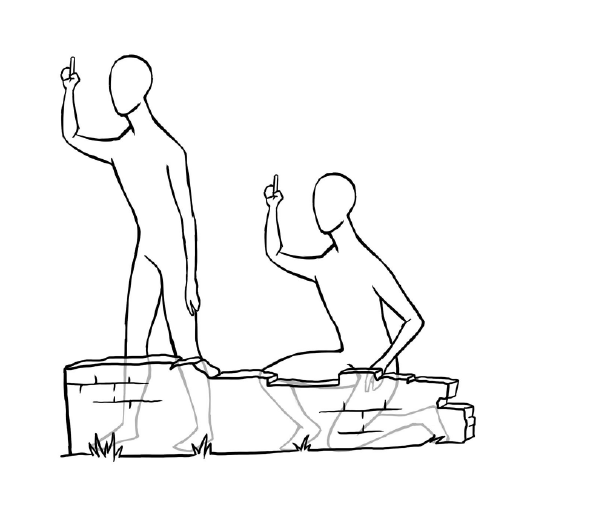
\includegraphics[width=1\textwidth]{images/image2.png}Appendix I. Stealth Cover Diagrams

\textbf{Figure 1}: using low walls as cover for the Stealth skill. \textbf{Neither} of these people are in stealth, as the low wall does not cover at least 50\% of their size from at least one side. They would need to position themselves lower for the wall wall to provide sufficient cover.

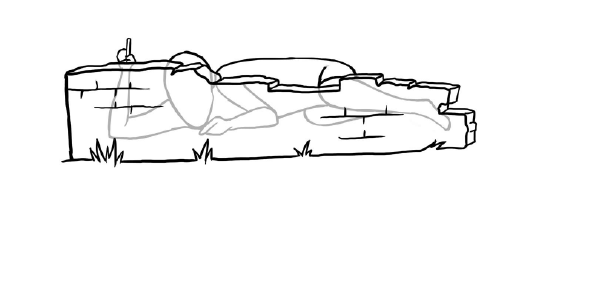
\includegraphics[width=1\textwidth]{images/image3.png}\textbf{Figure 2}: using low walls as cover for the Stealth skill. This person is in stealth, as the low wall now covers at least 50\% of their size from at least one side.

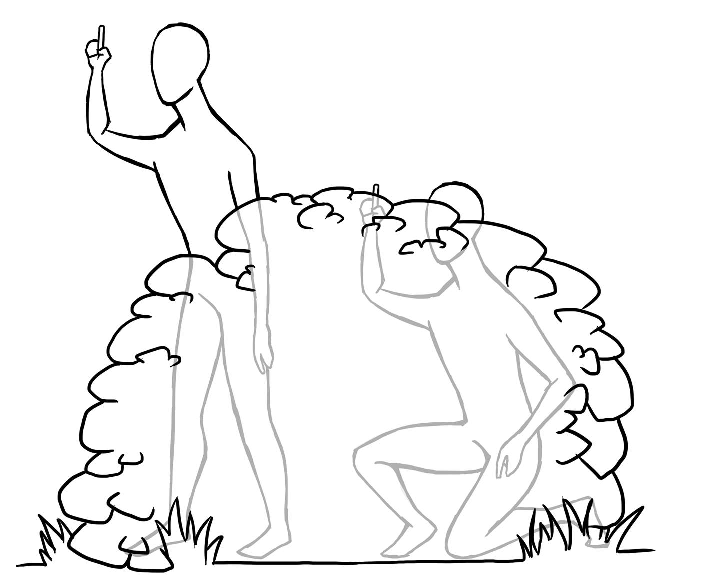
\includegraphics[width=1\textwidth]{images/image4.png}

\textbf{Figure 3}: using bushes and mid-level undergrowth for the Stealth skill. The person on the left is \textbf{not} in stealth, as they are standing upright instead of crouched, even though the bush covers at least 50\% of their size. The figure on the right is in stealth, as they are crouching behind the bush.

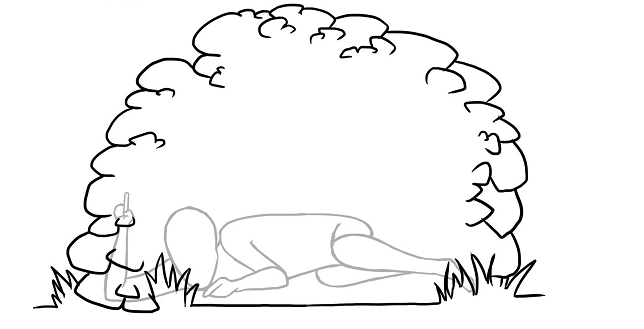
\includegraphics[width=1\textwidth]{images/image5.png}

\textbf{Figure 4}: using bushes and mid-level undergrowth for the Stealth skill. This person is in stealth. Although just crouching would provide sufficient cover behind this bush, the person has chosen to lie down - another valid way to place yourself in stealth.


\includegraphics[width=1\textwidth]{images/image6.png}

\textbf{Figure 5}: using trees and taller undergrowth for the Stealth skill. The person in the top left is \textbf{not} in stealth, as although the undergrowth here provides more than 50\% cover they are standing, and must be crouched or lower for it to count as stealth. The other two figures are both in stealth, as the undergrowth provides more than 50\% coverage of their size from at least one side, and they are in a crouched position or lower.

\textbf{Appendix J.} \textbf{\textit{Blastersmiths UK}} \textbf{Blaster Safety Guidelines}

\subsection{Blaster Standards}

In the interests of openness and fairness, we have laid out the standards that all blasters must adhere to, either mechanically or electrically.

Physical condition

Sharp edges and cracked plastic are not permitted: while melee striking and blocking with a blaster are banned, accidents can happen, therefore a blaster should not have sharp edges that may accidentally harm a person in this situation. Blasters that use a spring to provide power should be inspected for signs of stress if the spring has been upgraded. Particular areas of stress will be highlighted by white stress marks in the ABS plastic.

Firing capability

The blaster must be able to fire approved ammunition (see point \textit{2.2 Dart Types}) at a target. Whether or not it hits the target is irrelevant.

Muzzle velocity

The system uses a chronograph to measure the velocity (speed) of darts when they leave the muzzle of a blaster. The upper limit is 130 feet per second (39.62 metres per second). For comparison's sake, a stock (unmodified) Nerf Retaliator fires at about 65 feet per second (19.81 metres per second).

Wiring standards

The standards require that all joins are insulated with either heat shrink tubing (HST, preferred) or electrical tape. Hot glue insulation is not permitted. If a blaster has been rewired by a system-approved outfit (currently either \textit{Blastersmiths UK} or \textit{UKNerfWar}) then it passes the wiring safety standards. Otherwise, photos of the internals must be presented to the safety checker. If no such photos are available, the blaster will be opened by the player and inspected by the safety checker to ensure compliance. Blasters that are not electrical (or only have a small integrated torch, eg the Firestrike), or electrical blasters that are not modified, do not need to be opened. Evidence of intact seals may be required in order to verify modification status.

Battery standards

All batteries should be within a hard plastic case - typically the blaster's battery tray. A pack of silica gel (which absorbs moisture) is strongly recommended to ward against condensation and light rain.

\textit{AA alkalines, NiMH rechargeables and similar}

These cells should in good condition and not be leaking. In the case of NiMH, each cell should read roughly 1.2V while alkalines should read 1.5V. Often, white crusting or similar discolouration will indicate a problem with a battery. Any batteries in poor condition must be replaced in order for the blaster to be deemed safe.

\textit{TrustFire}

Extra care must be taken when handling TrustFire batteries: they are safe for use in the system but with a number of caveats. The only permitted brand of TrustFire battery is the ocial, silver-wrapped version.

Ultrareds and non-branded cells are not permitted. They must be checked after every engagement for symmetry of discharge - in other words that each battery has the same voltage. If they don't, they need to be charged. Nominal voltage should be 3.7V. Cells presenting at 3.4V or below need to be charged.

\textit{NiMH, NiCd and lithium battery Packs}

These must be checked for leakage and/or swelling. Lithium packs must have a voltage monitoring system

either a voltmeter, or an RC battery alarm. We recommend wrapping lithium packs in bubble wrap within the blaster's battery tray for extra protection against impacts. Lithium packs must read at least a voltage of 3.4V/cell (lithium polymer) or 3V/cell (lithium iron phosphate/LiFePO4).

\subsection{Ammunition Types}

Dart tip guide

Hard, dense-tipped full vinyl jacket (or ``FVJ'') darts are banned in the system. Without eye protection, these darts pose a serious risk of injury due to their dense, solid tip.

Dart types

Players are allowed to use the following dart types. There may often be a colour variant to tip types.

\textit{Off-the-shelf Hasbro darts}

\begin{itemize}
\item Orange ``streamlines'' - these are old, and no longer for sale, but are still permitted.

\item Blue ``elites'' - these are Hasbro's current ammo standard.

\item Various ``whistler'' darts - these have a large rubber head and only function in certain pistol-sized blasters. Also old, and no longer sold.

\item Various ``tagger'' darts - these have large rubber heads and velcro on their tips. Also old, hard to come by.

\item Various ``suction'' darts - Hasbro supplies two types of suction cup dart, the older Micro Suction dart and the new, blue-bodied Universal Suction Dart.

\item Various recoloured ``elite'' darts from sub-lines - eg Zombie Strike and Rebelle.

\item Mega Darts - Hasbro's newer and larger ammo type.

\end{itemize}
\textit{Aftermarket darts}

\begin{itemize}
\item ``Koosh'' darts - have a rough-looking head.

\end{itemize}
Specifically banned ammunition

Ammunition not discussed above is not permitted for use, such as Vortex (``XLR'') discs and Rebelle Arrows. All darts must be produced by an OEM manufacturer, home-made darts or modied darts are banned for use within the system. This includes, but isn't limited to, glue domes, UBER-domes and metal weighted stefans. ``Voberry'' darts / ``Voberries'' are specifically banned due to their harder heads.

Appendix K. Disclaimer

\subsection{Disclaimer}

At the site there is a variety of terrain such as woodland, fields and glades; we at \textit{Trinity Games} have done all we reasonably can to provide a safe environment for people to move in. However, due to the nature of the terrain \textit{Trinity Games} cannot be held responsible for any injuries sustained as a result of moving over the terrain. Being sensible about how people move over terrain is the sole responsibility of the individual, and by signing this form you state that you understand and agree to this at all times while you are on site. As such, \textit{Trinity Games} cannot be held accountable for any injuries sustained as a result of the terrain.

Due to the site being shared with other people in different areas, and any dangerous areas we are trying to safeguard against, any cordoned off areas are not to be entered.

On the site it is the responsibility of the individual to lift their own items, put up their own tents and transport their own kit that they have brought with them. The individual needs to judge whether they are fit/strong enough to be able to lift / manually handle any items of their own or anything else they choose to handle.

It is the responsibility of the individual to be able to judge any physical movements or lifting, and \textit{Trinity Games} cannot be held accountable for any injuries sustained as a result of improper lifting and handling of objects.

If you sustain an injury, \textit{Trinity Games} will do everything they can to help, and have risk assessments in place to try to safeguard against injuries. If you sustain an injury on site, we ask that you report it to a referee, Game Organisation Desk (GOD) or one of the team, so that a first aider can look at your injury and help where possible. If the first aider assesses that the injury needs more medical attention than has/can be given on site, you may taken to a medical facility, either by private transport or by ambulance if the first aider considers it necessary. Should this occur procedures are in place to safeguard your belongings left on-site.

It is the responsibility of the individual to make sure they are suitably nourished and hydrated while on site. Although every effort will be made to ensure running water and catering will be available on-site, there may be occasions where this is not possible, and due notice will be given in advance of events.

We often have a licensed bar on-site for adults (anyone suspected to be under the age of 18 will be asked to show identification as proof of age). If anyone is considered to be drinking excessively, having fun at the expense of other people, undertaking any illegal activity, bullying, or being too loud and/or obnoxious, then they may be spoken to by members of the team, possibly asked to leave site, and, if circumstances deem it necessary, asked not to return. \textit{Trinity Games} are here to ensure everyone has fun in a safe way. By signing this you agree to the team's decisions on any events that may cause an issue.

Anyone in a high-vis jacket bearing the \textit{Green Cloaks} logo on-site is considered to be a staff member of \textit{Trinity Games} and should be treated with respect. Sometimes they may be asked to communicate with you regarding important matters which will have been discussed by the team and passed on by them, or they may be communicating to you for your own best interest. They may also issue instructions in the case of emergency and other aspects of the game, and in this instance you are expected to follow instructions. If anyone is seen to be abusive to a member of staff they will be asked to leave the site. By signing this document you declare that you understand and agree to this.

Rules are in place to ensure safe areas, safety on site, fair play, fun and adventure. If you wish to discuss any matters with a member of the team, please send us an email at \textbf{trinitygames@hotmail.com} and we will happily discuss any issues you have concerns with.

137

Appendix L. Parent / Guardian Consent Form

If you are under the age of 18, in order to take part within games organised by \textit{Trinity Games}, this parent/

guardian consent form needs to be filled out and signed by your parent or guardian.

You, the player, must also fill out and sign the document to say that you have read the Disclaimer, that you

have understood it, and that you will adhere to its stated rules while on site.

Parent / Guardian

By signing this document you declare you have read through the Disclaimer, understand what has been said, agree to allow to your child to attend, and that they understand and agree to adhere to the rules.

\begin{table}
\begin{tabular}{|l|l|} \hline 
\textbf{Name of parent / guardian (printed)} &  \\
 \hline \textbf{Address} &  \\
 \hline \textbf{Postcode} &  \\
 \hline \textbf{Phone number} &  \\
 \hline \textbf{Signed} &  \\
 \hline \textbf{Date} &  \\
 \hline \end{tabular}

\end{table}

Emergency contact

\begin{table}
\begin{tabular}{|l|l|} \hline 
\textbf{Name} &  \\
 \hline \textbf{Relationship to player} &  \\
 \hline \textbf{Emergency contact number} &  \\
 \hline \end{tabular}

\end{table}

\textbf{Player}

By signing this document you declare you understand and agree to adhere to the rules that are in place and accept the team's judgment and decisions when made. You also agree to behave in a socially acceptable manner without issue.

\begin{table}
\begin{tabular}{|l|l|} \hline 
\textbf{Name} &  \\
 \hline \textbf{Signed} &  \\
 \hline \textbf{Date} &  \\
 \hline \end{tabular}
\end{table}
